


\documentclass[12pt,letter,titlepage]{article}
% pour d\'efinir les caract\'eristiques g\'en\'erales du document
%!TEX TS-program = pdflatexmk
\usepackage[latin1]{inputenc}
\usepackage[T1]{fontenc}
\usepackage{amsfonts}
\usepackage{amsmath}
\usepackage{graphicx}
\usepackage{natbib}
\usepackage{listings}
\usepackage[toc,acronym]{glossaries}
\usepackage{hyperref}
\usepackage[usenames,dvipsnames]{xcolor}
\makeglossaries
\usepackage{fancyhdr}
\setlength{\headheight}{15.2pt}
\pagestyle{fancyplain}
\usepackage{pdfpages}
\usepackage{listings}
\usepackage{color}
\usepackage{tabto}

\definecolor{dkgreen}{rgb}{0,0.6,0}
\definecolor{gray}{rgb}{0.5,0.5,0.5}
\definecolor{mauve}{rgb}{0.58,0,0.82}

\lstset{ %
  language=python,                % the language of the code
  basicstyle=\ttfamily,           % the size of the fonts that are used for the code
  numbers=left,                   % where to put the line-numbers
  numberstyle=\tiny\color{gray},  % the style that is used for the line-numbers
  stepnumber=2,                   % the step between two line-numbers. If it's 1, each line 
  % will be numbered
  numbersep=5pt,                  % how far the line-numbers are from the code
  backgroundcolor=\color{white},      % choose the background color. You must add \usepackage{color}
  showspaces=false,               % show spaces adding particular underscores
  showstringspaces=false,         % underline spaces within strings
  showtabs=false,                 % show tabs within strings adding particular underscores
  rulecolor=\color{black},        % if not set, the frame-color may be changed on line-breaks within not-black text (e.g. commens (green here))
  tabsize=2,                      % sets default tabsize to 2 spaces
  captionpos=b,                   % sets the caption-position to bottom
  breaklines=true,                % sets automatic line breaking
  breakatwhitespace=false,        % sets if automatic breaks should only happen at whitespace
  title=\lstname,                   % show the filename of files included with \lstinputlisting;
}

\newcommand{\specialcell}[2][c]{%
  \begin{tabular}[#1]{@{}c@{}}#2\end{tabular}}

\def\mytitle{CO250 :Assignment 1}
\title{\mytitle}
\definecolor{gray}{rgb}{0.3,0.3,0.3}
\hypersetup{linkbordercolor={1 1 1},
  colorlinks=true,
  linkcolor=gray}
\setcounter{tocdepth}{2}


\author{Bastien Jacot-Guillarmod, Christian Zommerfelds}
\lhead{Bastien Jacot-Guillarmod, Christian Zommerfelds}
\rhead{\today}


%%%%%%%%%%%%%%%%%%%%%%%%%%%%%%%%%%%%%%%%%%%%%%%%%%%%%%%%%%%%%%%%%%%%%%%%%%%%%%%%%%%%%%%%%%%%%%%%%%%%%%%%%%%%%%%%%%%%%%%%%%%%%%%
%%%%%%%%%%%%%%%%%%%%%%%%%%%%%%%%%%%%%%%%%%%%%%%%%%%%%%%%%%%%%%%%%%%%%%%%%%%%%%%%%%%%%%%%%%%%%%%%%%%%%%%%%%%%%%%%%%%%%%%%%%%%%%%

\begin{document}

\begin{center}
  {\bf \Large 
    ECE 458 - Project Proposal\\
   \LARGE
    OIS: Online Initiative System\\
    %A Secure `We, the People'
  }
\end{center}
\vspace{0.2cm}

{\bf Team Members}
\vspace{0.1cm}

\noindent Bastien Jacot-Guillarmod \tabto{6cm} 20493646 \\
\noindent Christian Zommerfelds    \tabto{6cm} 20493973

%%%%%%%%%%%%%%%%%%%%%%%%%%%%%%%%%%%%%%%%%%%%%%%%%%%%%%%%%%%%%%%%%%%%%%%%%%%%%%%%%%%%%%%%%%%%%%%%%%%%%%%%%%%%%%%%%%%%%%%%%%%%%%%
%%%%%%%%%%%%%%%%%%%%%%%%%%%%%%%%%%%%%%%%%%%%%%%%%%%%%%%%%%%%%%%%%%%%%%%%%%%%%%%%%%%%%%%%%%%%%%%%%%%%%%%%%%%%%%%%%%%%%%%%%%%%%%%

\section{Abstract}
We propose to implement a secure governmental website, to enable citizens of the country to sign popular initiatives in a secure way. It should provide protection mechanisms to ensure the same level of security as traditional pen and paper systems.

\section{Problem Statement}
As two Swiss citizens, we became interested in the idea of implementing a system that could be used by Switzerland's government to help voters to sign popular initiatives online. In Switzerland, the law allows citizens which are entitled to vote to create popular initiatives to make changes to the constitution. If the number of signatures reaches 100,000, the initiative will be put to a referendum, where the whole country will vote to decide whether the proposal will be accepted or rejected.

Another interesting example is `We, the People', a petition system created by the White House that allows U.S. citizens to create and sign petitions online. Even if this is a great solution to increase the communication between taxpayers and the government, it is not suitable for initiatives. For instance, a non-U.S. citizen can easily create an account and sign petitions. Therefore, there is a need for a stricter protocol to ensure the indentity of a real voter.

We want to create our system providing a generic solution, but keeping the Swiss government in mind to create a realistic problem with different levels of requirements. We will try to create a system which can work side by side and collaborating with the pen and paper system. Thus we need a tool to verify that a citizen did not sign the same bill twice, once online and once physically. In Switzerland the municipality is responsible for checking if one of his inhabitants did not sign the same draft more than once. With our system, they would need to have access to the federal database of petition signatures to ensure the citizen did not use both means of signing.

It might also be useful for the initiative comitee (i.e. the people who drafted the bill) to access the database in a way they can gather informations on their proposal, such as number of signatures, deadlines, demographics tendencies, etc...


\section{Our Solution}
We propose to create a web application in a test environment which will provide the software prototype for such a system. A part of the registration process would not be electronic, therefore we will only plan this part and not implement it.

\subsection{Design}
As shown on figure \ref{diag}, the registration process has to involve the administration to ensure that the inquiring user is a real citizen and does not already have an account. To avoid an identity theft, the log-in procedure should then be sent offline to the voter, for instance by registered letter containing the username and password. The user can access the list and description of each initiative without logging in, but would need to provide this data to be able to sign any bills.

An interesting part of our project will be to design the different access roles of the federal and local administrations. This will have to be done maximizing privacy and security.

\begin{figure}

\begin{center}
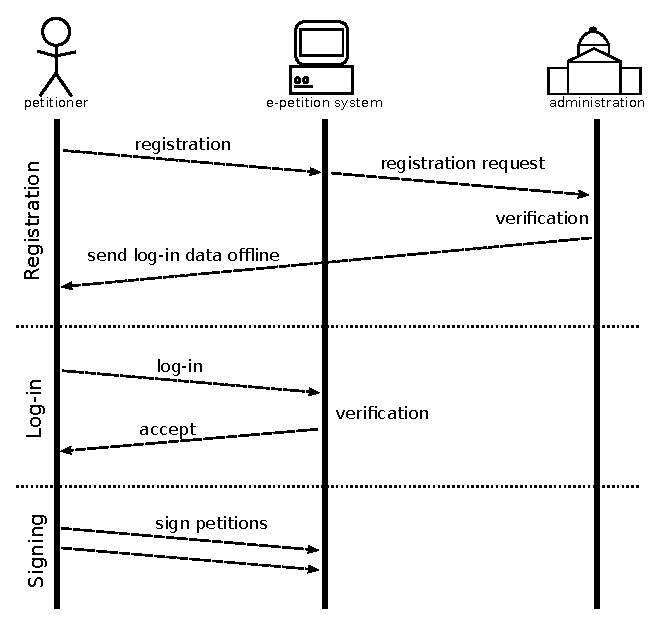
\includegraphics[width = 0.9 \textwidth]{drawing.eps}  
\end{center}  
  \caption{Diagram illustrating the interaction between the voter and the system.}
  \label{diag}
\end{figure}



 \subsection{Implementation}
We will use a secure protocol such as HTTPS to establish an encrypted connection between the voters and the server.

A database will be managed by the web application. We will use a TomCat Server, which is implemented with MySQL, Java and JSP. We will need to protect the privacy of each user, therefore we will split each role in such a way that they can only access the minimum data needed. Parts of our system will be testable using JUnit tests. We'll try to keep our system as modulable as possible and write unit tests for the back-end Java code. But for a big part we'll have to rely on human testing directly on the website's interface. For the most part, only us two will act as testers. But if the necessity arises, we'll ask external people to test our system.

For the development we will create our own certificate for our website and add it to our web-browser. Our assumption is that the organization using our software would get a certificate from a major issuer that is already known to modern browsers.

\section{End-to-end Security Analysis}
Our system will be reasonably secure against Man-in-the-middle attacks by implementing authentication of our web site. The TLS protocol (used by HTTPS) will help us to make this implementation.

Additionally, because TLS allows bidirectional encryption of communications between a client and server, our system would be protected against eavesdropping and tampering.

Of course there are many potential security issues to be considered. The interface between the online system and the organization entities can be a major source of security problems. For example, an officer with bad intentions and access to the database could try to modify the collected data. The authentication process for the administrative organs has to be secure enough to ensure privacy and integrity of the data. Hence the organization using our system would have to establish internal policies for the access to the system. Ideally, the number of people who have access to the full data has to be kept to a minimum. We can address this problem by making our system manage the distribution of the signatures to the respective home cities. This way, all the output that the administration office needs from our system is how many signatures were collected.

One security problem that remains open is identity theft by stealing a person's log-in data (e.g. by having physical access to the registration response letter). One way to solve this problem would be to use bio-metric data for authentication. But we believe that the currently defined level of security of the system is enough for the purposes of initiative signing and roughly equivalent to traditional pen signatures methods.

\section{Usability Issues}
To avoid identity theft and to strenghten the security of the system, we will most likely make use of some physical communication system, which add a big delay to the registration process. Since most of the citizens are reluctant to participate in politics, specially if some administration is involved, this issue can be the biggest barrier to the success of our idea.

One other obstacle can also be the fear of the `Big Brother'. Some could see an electronic database of the citizens as a mean to hinder the freedom of the people. Against such antipathy, the only possibility is to keep the pen and paper system running to allow an alternative to our approach of the problem and only store data from citizens that are willing to use the electronic system.

\section{References}

\subsection*{We, the People}

\url{https://petitions.whitehouse.gov/how-why/introduction}

\subsection*{Popular Initiatives in Switzerland}

\url{http://en.wikipedia.org/wiki/Initiative#Switzerland}\\
\url{http://de.wikipedia.org/wiki/Volksinitiative_(Schweiz)}
 

\subsection*{TomCat Server}
\url{http://tomcat.apache.org/}

\end{document}
